\documentclass[10pt,english]{article}

\usepackage{geometry}
\geometry{verbose,letterpaper,tmargin=1in,bmargin=1in,lmargin=1in,rmargin=
1in}
\usepackage{helvet}
\usepackage[T1]{fontenc}
\usepackage[latin1]{inputenc}
\usepackage{setspace}
\usepackage{paralist}
\usepackage{color}
\usepackage{hyperref}
 \hypersetup{backref,colorlinks=true}
\usepackage{ae,aecompl}
\usepackage{graphicx}
\usepackage{picins}
\usepackage{fancyhdr}
\usepackage{extramarks}
\pagestyle{empty}
%define tip float
\usepackage{float}
\floatstyle{ruled}
\newfloat{Tip}{H}{lox}
\floatname{Tip}{Tip}
\newcommand\qgistip[1]{\raggedright\small{#1}}
\renewcommand{\topfraction}{0.85}
 \renewcommand{\textfraction}{0.1}
\renewcommand{\floatpagefraction}{0.75}

%\renewcommand\familydefault{lucidabrightsans}
\title{Quantum GIS User Guide\\
\large Version 0.5 \textsl{'Bandit'}}
\author{Gary E. Sherman \\Tim Sutton (Rasters) \\Radim Blazek (GRASS)}
%\date{\small July 2004}

\begin{document}


% To disable first line indents of paragraphs after the first one
\setlength{\parindent}{0in}


\maketitle
\tableofcontents
\listof{Tip}{QGIS Tips}
%\newpage

%\fancyfoot[C]{\thepage}
\pagestyle{fancy}
\fancyhead[L]{QGIS User Guide}
\fancyhead[R]{\textsl{Version 0.5}}


\begin{onehalfspace}
\reversemarginpar
\section{Introduction}
Quantum GIS (QGIS) is designed to be a Geographic Information System
(GIS) built for Linux/Unix, Mac OSX, and Windows. QGIS currently offers basic support for
vector (both disk-based and database) and raster formats. 

QGIS is released under the GNU Public License. You should have received a full copy of the license with your copy of QGIS.
\begin{quote}
\begin{singlespace}
\textsl{Note - The latest version of this document can always be found at\\
http://qgis.sourceforge.net/docs/userguide.html }
\end{singlespace}
\end{quote}
\section{Whats New in 0.5}
New features in version 0.5 include:
\begin{compactenum}
\item Windows version
\item Feature labeling with optional buffering
\item Preliminary digitizing support for shapefiles
\item GRASS digitizing support
\item GPS SVG icons
\item Unique value renderers
\item User interface improvements
\item Specify a query when loading a PostGIS layer
\item Italian translation

\end{compactenum}
\section{Major Features}

QGIS has many common GIS features and functions. The major features
are listed below. 

\begin{compactenum}
\item Support for spatially enabled PostgreSQL tables using PostGIS 
\item Support for ESRI shapefiles and other vector formats support by the
OGR library, including MapInfo files 
\item Identify features 
\item Display attribute table 
\item Select features 
\item Label features
\item Persistent selections 
\item Save and restore projects
\item Support for raster formats supported by the GDAL library 
\item Change vector symbology (single, graduated, unique value, and continuous) 
\item SVG markers symbology (single, unique value, and graduated) 
\item Display raster data such as digital elevation models, aerial photography
or landsat imagery 
\item Change raster symbology (grayscale, pseudocolor and multiband RGB) 
\item Export to Mapserver map file 
\item Preliminary digitizing support
\item Map overview
\item Plugins 
\end{compactenum}

\section{Getting Started}

This section gives you a quick overview of running QGIS and examining
data available on the QGIS web page.


\subsection{Installation}

Installation of QGIS is documented in the Installation Guide. The Installation Guide is distributed with the QGIS source code and is also available at \url{http://qgis.org}.


\subsection{Sample Data}

If you do not have any GIS data handy, you can obtain a dataset for Alaska from the QGIS web site at \url{http://qgis.org}. The Alaska data set will be used as the basis for the examples and screenshots provided in this document.


\subsection{Starting QGIS}

Assuming that QGIS is installed in the PATH, you can start QGIS by
typing: \textbf{qgis}  at a command prompt or by double clicking on the QGIS application link (or shortcut) on the desktop.
%\begin{figure}
%\caption{QGIS Main Window}
%\end{figure} 
\begin{Tip} \caption{\textsc{Using command line arguments}}
\qgistip{
You can also start QGIS by specifying one or more datafiles
on the command line. For example, assuming you are in your data directory,
you could start QGIS with two shapefiles and a raster file set to
load on startup using the following command: 
\ttfamily{	qgis ak\_shade.tif alaska.shp majrivers.shp}
}
\end{Tip}

\subsection{The QGIS Main Window}
When QGIS starts, an empty window is displayed as shown below.

\begin{figure}[h]
   \begin{center}
   \caption{Main window}\label{fig:startup}
   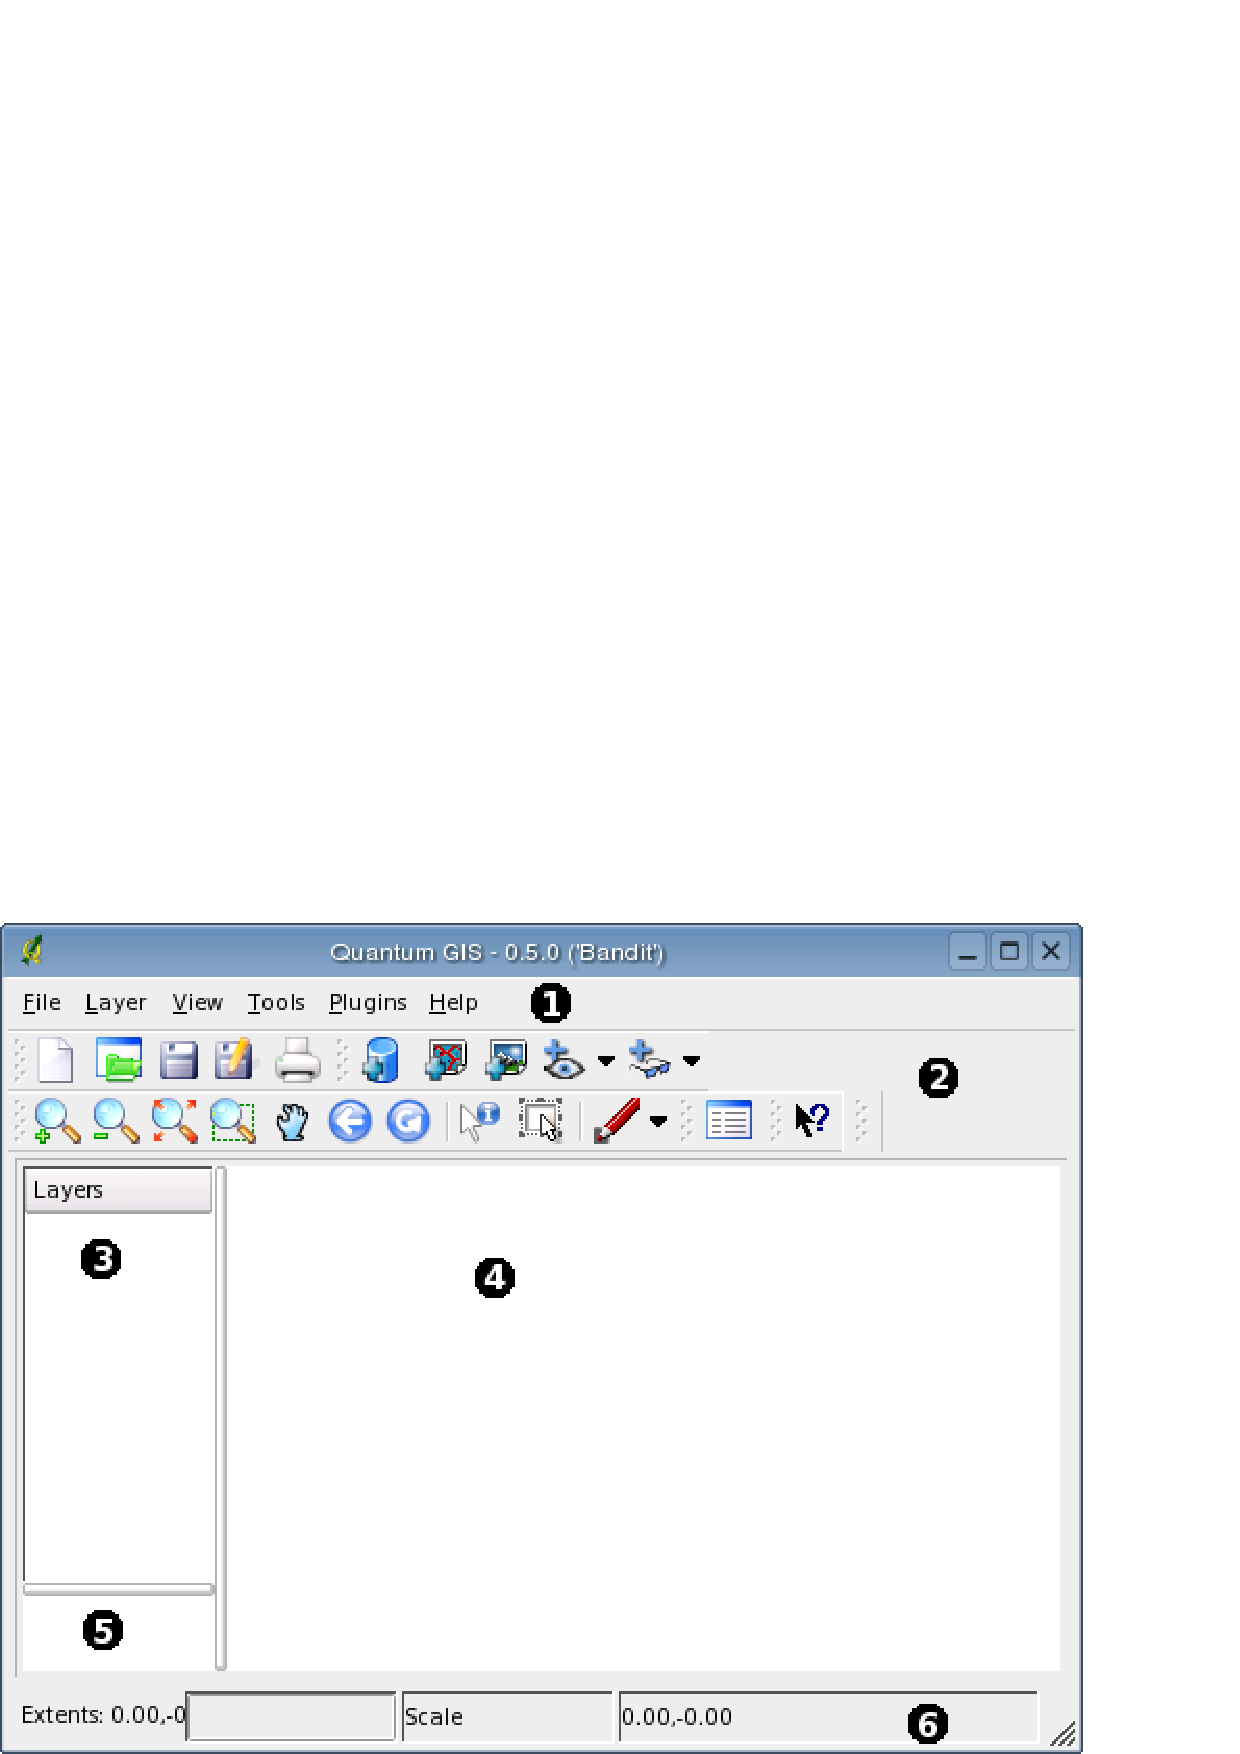
\includegraphics[scale=.9]{qgis_user_guide_images/startup}
\end{center}  
   
\end{figure}
\
textsc{Note - Your window decorations (title bar, etc.) may appear different depending on your operating system and window manager}
The QGIS main window is divided into five areas:
\begin{compactenum}
\item The menu bar
\item The tool bar
\item The map legend
\item The map view
\item The map overview
\item The status bar
\end{compactenum}

These six components of the QGIS interface are described in more detail in the following sections
\subsubsection{The QGIS menu bar}

The menu bar provides access to various QGIS features using a standard windows
heirachical menu. The top-level menus and a summary of some of the functions provided are:
\begin{compactitem}
\item File (project open, save, export image, properties)
\item Layer (add, show, hide layers)
\item View (zoom, refresh)
\item Tools (plugin manager, preferences)
\item Plugins (menus added by plugins as they are loaded)
\item Help (documentation and web links)
\end{compactitem}
%See Appendix \ref{app_menu} for complete descriptions of the menu items.

\subsubsection{Toolbars}
The toolbars provide access to most of the same functions as the menus, plus
additional tools for interacting with the map. Each toolbar item has popup
help available. Hold your mouse over the item and a short description of the
tool's purpose will be displayed. %See Appendix \ref{app_toolbar} for complete
%descriptions and illustrations of the various toolbars.  

\subsubsection{The QGIS map legend}
The map legend area is used to set the visibility and z-ordering of layers.
Z-ordering means that layers listed nearer the top of the legend are drawn
over layers listed lower down in the legend. The checkbox in each legend entry
can be used to show/hide that layer.
\begin{Tip} \caption{\textsc{Viewing the Layer Menu}}
\qgistip{You can display the context menu for any layer in the legend by right-clicking
on the layer name. The context menu contains items for working with the layer and viewing
its properties.}
\end{Tip}

\subsubsection{The QGIS map view}

This is the 'business end' of QGIS - maps are displayed in this area! The map
displayed in this window will depend on the vector and raster layers you have
chosen to load (see sections that follow for more info on this). The map view
can be panned (shifting to focus of the map display to another region), zoomed
in and out, and supports various other actions as described in the toolbar
description above.  The map view and the legend are tightly bound to each
other - the maps in view reflect changes you make in the legend area.  
\begin{Tip}\caption{\textsc{Zooming the Map with the Mouse Wheel}}
\qgistip{You can use the mouse wheel to zoom in and out on the map. Place the mouse cursor inside the map area and roll it forward (away from you) to zoom in and backwards (towards you) to zoom out.
}
\end{Tip}
\subsubsection{The QGIS map overview}
The map overview area provides a full extent view of layers added to it. Within the view is a rectangle showing the current map extent. This allows you to quickly determine which area of the map you are currently viewing.

\subsubsection{The QGIS map status bar} 
The status bar shows you your current position in map coordinate (e.g. meters
or decimal degress) as the mouse pointer is moved accross the map view.

\section{Working with Vector Data}
QGIS supports vector data in a number of formats, including shapefiles,
MapInfo mif, and PostGIS layers in a PostgreSQL database. Support for
additional data types is provided by plugins, for example delimited text.\\

This section describes how to work with two common formats: shapefiles and
PostGIS layers. Many of the features available in QGIS work the same regardless of the 
vector data source. This is by design and includes the identify, select, labeling, and attributes functions.

\subsection{Shapefiles}
Shapefile support is provided by a library of functions (OGR \url{http://www.remotesensing.org/gdal/ogr}). See Appendix \ref{appdx_ogr} for a list of supported formats.\\

A shapefile actually consists of a minimum of three files:
\begin{compactenum}
\item .shp file containing the feature geometries
\item .dbf file containing the attributes in dBase format
\item .shx index file
\end{compactenum}
The technical specification for the shapefile format can be found at\\ \url{http://www.esri.com/software/opengis/openpdf.html}.
\subsubsection{Loading a Shapefile}
\parpic[l]{
\includegraphics{qgis_user_guide_images/addshapefile}}To load a shapefile, start QGIS and click on the \textit{Add a vector layer} toolbar bar button. This same tool can be used to load any of the formats supported by the OGR library.

Clicking on the tool brings up a standard open file dialog (Figure \ref{fig:openshapefile}) which allows you to navigate the file system and load a shapefile (or other supported data source). 
\begin{figure}[h]
   \begin{center}
   \caption{Open OGR Data Source Dialog}\label{fig:openshapefile}\smallskip
   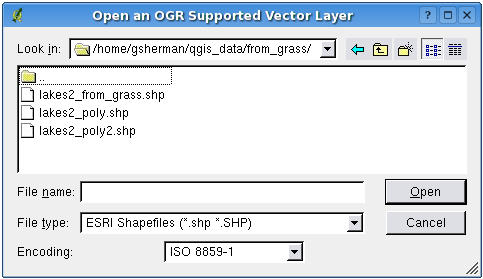
\includegraphics[scale=.75]{qgis_user_guide_images/shapefileopendialog}
\end{center}  
   
\end{figure}
Selecting a shapefile from the list and clicking Ok loads it into QGIS. Figure \ref{fig:loadedshapefile}
shows QGIS after loading the alaska.shp file.
\begin{figure}[h]
   \begin{center}
   \caption{QGIS with the Alaska Shapefile Loaded}\label{fig:loadedshapefile}\smallskip
   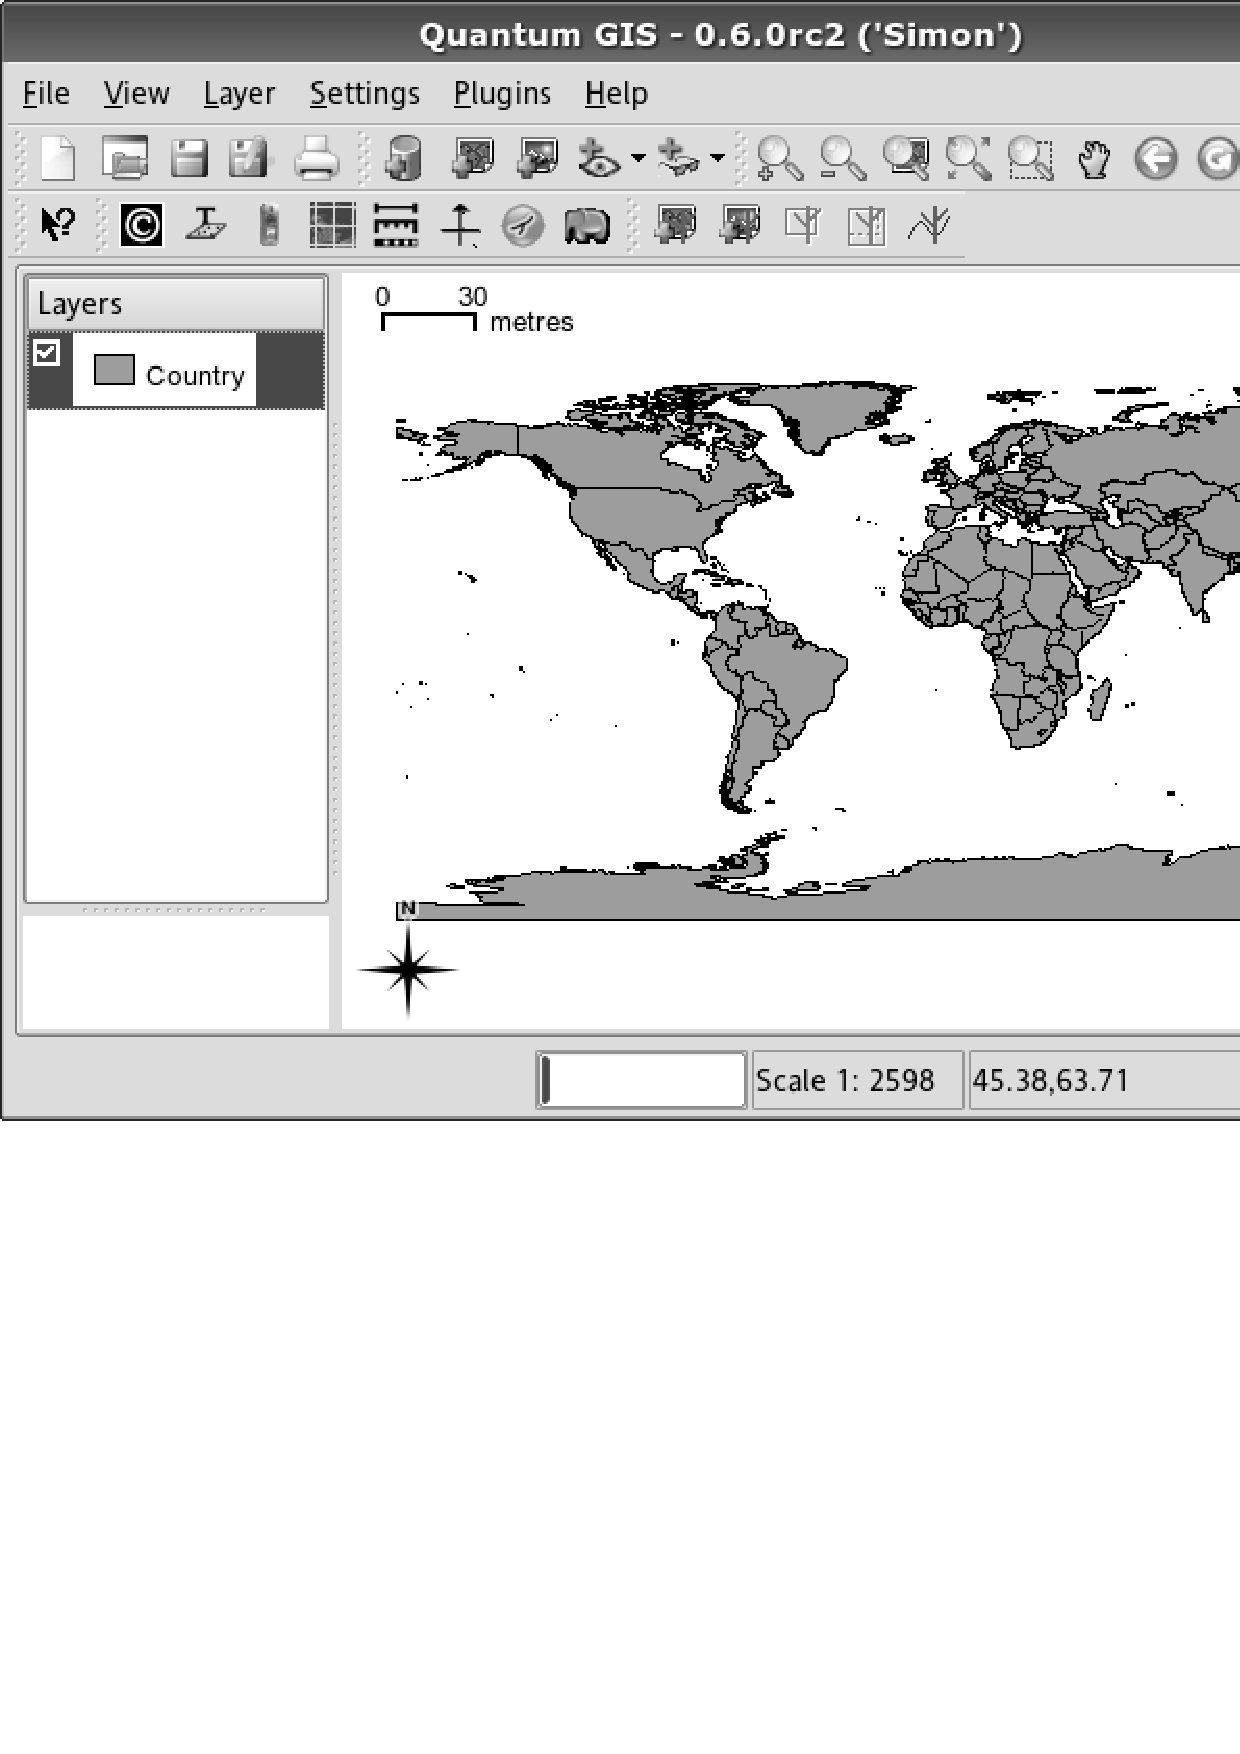
\includegraphics[scale=.6]{qgis_user_guide_images/shapefileloaded}
\end{center}  
   
\end{figure}
\begin{Tip}\caption{\textsc{Layer Colors}}
\qgistip{When you add a layer to the map, it is assigned a random color. When adding more than one layer at a time, different colors are assigned to each. }
\end{Tip}

Once loaded, you can zoom around the shapefile using the map navigation tools. To change the symbology of a layer, open the layer properties dialog by double clicking on the layer name or by right-clicking on the name in the legend and choosing \textsl{Properties} from the popup menu. See Section \ref{sec:symbology} for more information on setting symbology of vector layers.
\subsection{PostGIS Layers}
PostGIS layers are stored in a PostgreSQL database. The advantage of PostGIS is the spatial indexing, filtering, and query capability. Using PostGIS, vector functions such as select and identify work more accurately than with OGR layers in QGIS.
To use PostGIS layers you must:
\begin{compactenum}
\item Create a stored connection in QGIS to the PostgreSQL database (if one is not already defined)
\item Connect to the database
\item Select the layer to add to the map
\item Optionally provide a SQL where clause to define which features to load from the layer
\item Load the layer
\end{compactenum}
\subsubsection{Creating a Stored Connection}
\parpic[l]{
\includegraphics{qgis_user_guide_images/addpostgis}}The first time you use a PostGIS data source, you must create a connection to the PostgreSQL database that contains the data. Begin by clicking on the \textit{Add a PostGIS Layer} toolbar button. The \textsl{Add PostGIS Table(s)} dialog will be displayed. To access the connection manager, click on the \textsl{New} button to display the \textsl{Create a New PostGIS Connection} dialog. The parameters required for a connection are shown in Table \ref{tab:postgis_connection_parms}.
\begin{table}[h]
\centering
\caption{PostGIS Connection Parameters}\label{tab:postgis_connection_parms}\medskip
 \begin{tabular}{|l|p{5in}|}
\hline Name & A name for this connection. Can be the same as \textsl{Database} \\
\hline Host & Name of the database host. This must be a resolvable host name the same as would be used to open a telnet connection or ping the host \\
\hline Database & Name of the database  \\
\hline Port & Port number the PostgreSQL database server listens on. The default port is 5432.\\
\hline Username & User name used to login to the database \\
\hline Password & password used with \textsl{Username} to connect to the database\\
\hline
\end{tabular}
\end{table}
Once the parameters have been filled in, you can test the connection by clicking on the \textsl{Test Connection} button. To save the password with the connection information, check the \textsl{Save Password} option.
\begin{Tip}\caption{\textsc{QGIS User Settings and Security}}
\qgistip{Your customized settings for QGIS are stored based on the operating system. On Linux/Unix, the settings are stored in your home directory in .qt/qgisrc. On Windows, the settings are stored in the registry. Depending on your computing environment, storing passwords in your QGIS settings may be a security risk.
}
\end{Tip}
\subsubsection{Loading a PostGIS Layer}
\parpic[l]{
\includegraphics{qgis_user_guide_images/addpostgis}}Once you have one or more connections defined, you can load layers from the PostgreSQL database. Of course this requires having data in PostgreSQL. See Section \ref{sec:loading_postgis_data} for a discussion on importing data into the database. \\

To load a layer from PostGIS, perform the following steps:
\begin{compactenum}
\item If the PostGIS layer dialog is not already open, click on the \textit{Add a PostGIS Layer} toolbar button
\item Choose the connection from the drop-down list and click \textsl{Connect}
\item Find the layer you wish to add in the list of available layers
\item Select it by clicking on it. You can select multiple layers by holding down the shift key while clicking
\item Click on the \textsl{Add} button to add the layer to the map
\end{compactenum}
\begin{Tip}\caption{\textsc{Using a Definition Query with PostGIS Layers}}
\qgistip{If you wish to further define the features added from a PostGIS layer, double-click on the layer to open the SQL editor. Enter a conditional statement to be used to select features from the layer for display. For example, if you have a towns layer with a population field you could select only larger towns by entering \textsl{population > 100000}. Currently the SQL editor does not provide a list of field names to aid you in forming the conditional statement. The editor will be improved in a future release. Field names and values can be examined by loading the layer without a conditional statement and using the identify tool or by opening the attribute table.
}
\end{Tip}
\subsubsection{Importing Data into PostgreSQL}\label{sec:loading_postgis_data} 
Data can be imported into PostgreSQL using a number of methods. PostGIS includes a utility called shp2pgsql that can be used to import shapefiles into a PostGIS enabled database. \\

\parpic[l]{
\includegraphics{qgis_user_guide_images/spiticon}}QGIS comes with a plugin named SPIT (Shapefile to PostGIS Import Tool). SPIT can be used to load mutliple shapefiles at one time and includes support for schemas. To use SPIT, open the Plugin Manager from the Tools menu and load the plugin by checking the box next to the SPIT plugin and click Ok. The SPIT icon will be added to the plugin toolbar. \\

To import a shapefile, click on the SPIT tool in the toolbar to open the dialog. You can add one or more files to the queue by clicking on the \textsl{Add} button. To process the files, click on the Import button. The progress of the import as well as any errors/warnings will be displayed as each shapefile is processed.
\begin{Tip}\caption{\textsc{Importing Shapefiles Containing PostgreSQL Reserved Words}}
\qgistip{SPIT does not handle importing of shapefiles that contain field names that are reserved words in the PostgreSQL database. This issue will be addressed in a future release of the plugin
}
\end{Tip} 
\subsection{The Vector Properties Dialog}
The vector properties dialog provides information about a layer, symbology settings, and labeling options. To access the properties dialog, double-click on a layer in the legend or right-click on the layer and select Properties from the popup menu.

\subsubsection{Vector Symbology}\label{sec:symbology}

QGIS supports a number of symbology renderers to control how
vector features are displayed. Currently the following renderers
are available:

\begin{compactdesc}
    \item[Single symbol] - a single style is applied to every
    object in the layer.
    \item[Graduated symbol] - objects within the layer are
    displayed with different symbols classified by the values of a
    particular field.
    \item[Continuous colour] - objects within the layer are
    displayed with a spread of colours classified by the numerical
    values within a specified field.
    \item[Unique value] - objects are classified by the unique
    values within a specified field with each value having a
    different symbol.
\end{compactdesc}

For layers containing point features, additional renderers are
available that use SVG icons:

\begin{compactdesc}
    \item[Single marker] - a single specified icon is used for
    every point within the layer.
    \item[Graduated marker] - points within the layer are
    displayed with different icons classified by values within a
    particular field
    \item[Unique value marker] - points are classified by unique
    values within a specified field with each value having a
    different icon.
\end{compactdesc}


\section{Working with Raster Data}
QGIS supports a number of raster data formats. This section describes how to work with raster data in QGIS.
\subsection{What is raster data?}

Raster data in GIS are matrices of discrete cells that represent features on, above or below the earth's surface. Each cell in the raster grid is the same size, and cells are usually rectangular (in QGIS they will always be rectangular). Typical raster datasets include remote sensing data such as aerial photography or satellite imagery and modelled data such as an elevation matrix.\\

Unlike vector data, raster data typically do not have an associated database record for each cell.\\

In GIS, a raster layer would have georeferencing data associated with it which will allow it to be positioned correctly in the map display to allow other vector and raster data to be overlayed with it. QGIS makes use of georeferenced rasters to properly display the data.
	
\subsection{Raster formats supported in QGIS}
QGIS supports a number of different raster formats. Currently tested formats include:
\begin{compactitem}
\item Arc/Info Binary Grid
\item  Arc/Info ASCII Grid
\item Grass Raster
\item GeoTIFF
\item Spatial Data Transfer Standard Grids (with some limitations)
\item USGS ASCII DEM
\item Erdas Imagine
\end{compactitem}
Because the raster implmentation in QGIS is based on the GDAL library, other raster formats implemented in GDAL are also likely to work, but have not yet been tested. See Appendix \ref{appdx_gdal} for more details.
	
\subsection{Loading raster data in QGIS}
\parpic[l]{
\includegraphics{qgis_user_guide_images/addraster}}Raster layers are loaded either by clicking on the Load Raster icon or by selecting the View->Add Raster Layer menu option. More than one layer can be loaded at the same time by holding down the Control key and clicking on multiple items in the file dialog.\\
	
\subsection{Raster Properties}

\parpic[r]{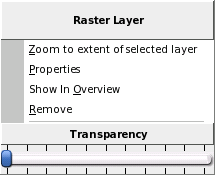
\includegraphics[scale=0.6]{qgis_user_guide_images/rastercontextmenu}}To view and set the properties for a raster layer, right click on the layer name. This displays the raster layer context menu that includes a number of items that allow you to:
\begin{compactitem}
\item Zoom to the full extent of the raster
\item Show the raster in the map overview window
\item Open the properties dialog (of course)
\item Remove the layer from the map
\item Set the transparency using a slider control
\end{compactitem}
Choose \textsl{Properties} from the context menu to open the raster properties dialog for the layer.\\


Figure \ref{fig:raster_properties} shows the properties dialog. There are four tabs on the dialog: \textsl{Symbology}, \textsl{General}, \textsl{Metadata}, and \textsl{Pyramids}.

\begin{figure}[h]
   \begin{center}
   \caption{Raster Layers Properties Dialog}\label{fig:raster_properties}\smallskip
   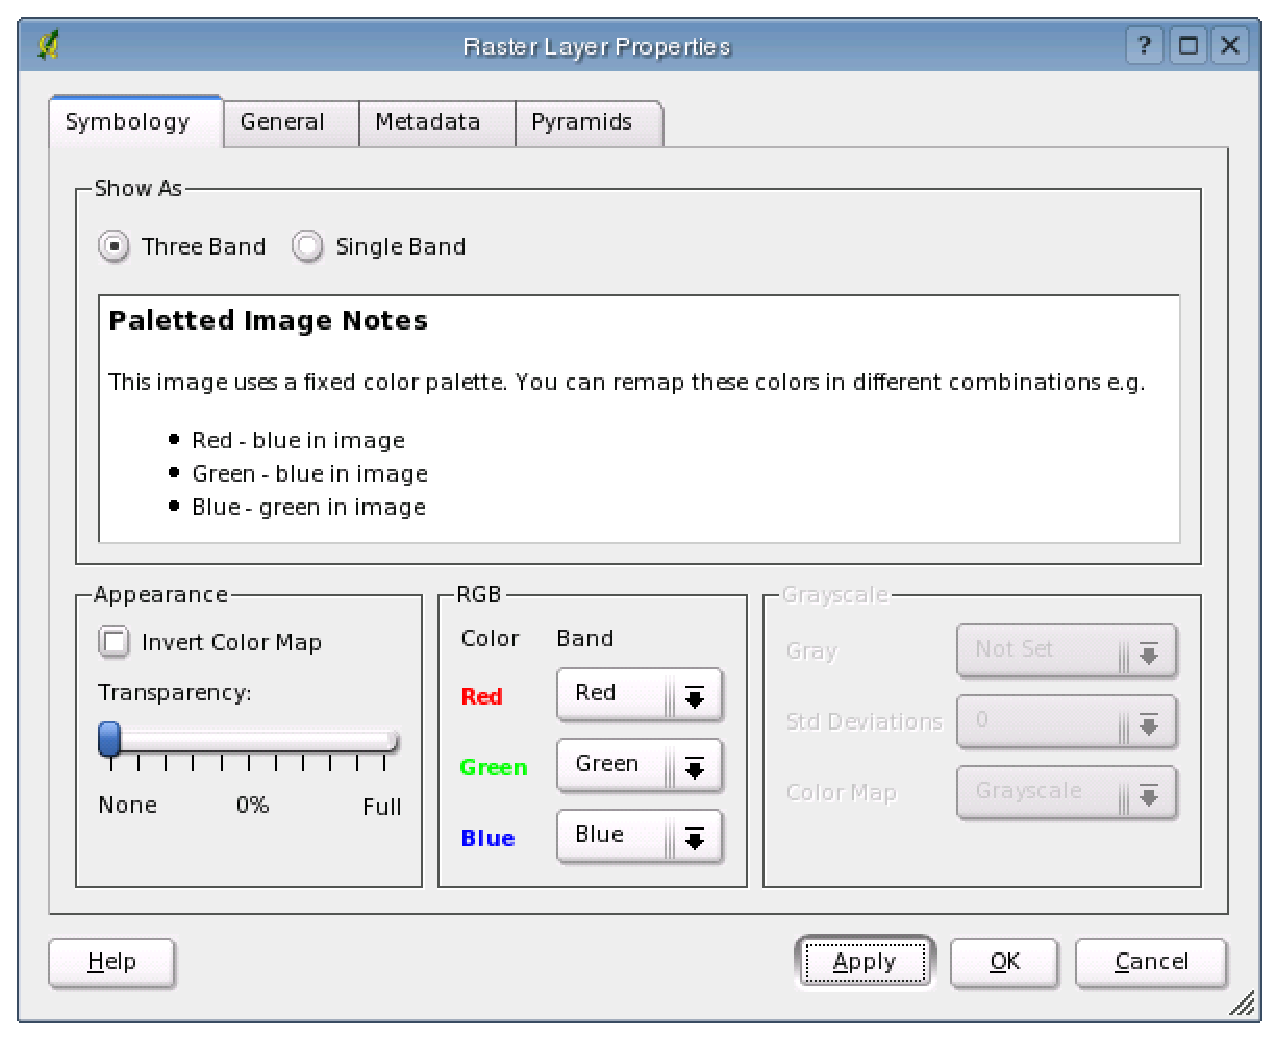
\includegraphics[scale=.7]{qgis_user_guide_images/raster_properties}
\end{center}  
\end{figure}


\subsubsection{Symbology Tab}


QGIS supports three forms of raster layers:
\begin{compactitem}
\item Single Band Grayscale Rasters
\item Palette Based RGB Rasters
\item Multiband RGB Rasters
\end{compactitem}

From these three basic layer types, eight forms of symbolised raster display can be used:
\begin{compactenum}

\item Single Band Grayscale
\item Single Band Pseudocolor
\item Paletted Grayscale (where only the red, green or blue component of the image is displayed)
\item Paletted Pseudocolor (where only the red, green or blue component of the image is displayed, but using a pseudocolor algorithm)
\item Paletted RGB
\item Multiband Grayscale (using only one of the bands to display the image)
\item Mulitiband Pseudocolor (using only one of the bands shown in pseudocolor)
\item Multiband RGB (using any combination of three bands)
\end{compactenum}
\smallskip
QGIS can invert the colors in a given layer so that light colors become dark (and dark colors become light). Use the \textsl{Invert Color Map} checkbox to enable / disable this behavior.\\

QGIS has the ability to display each raster layer at varying transparency levels. Use the transparency slider to indicate to what extent the underlying layers (if any) should be visible though the current raster layer. The transparency can also be set using the transparency slider in the layer context menu which is accessible by right-clicking on the layer in the legend.\\

QGIS can restrict the data displayed to only show cells whose values are within a given number of standard deviations of the mean for the layer. This is useful when you have one or two cells with abnormally high values in a raster grid that are having a negative impact on the rendering of the raster. This option is only available for pseudocolor images.\\

\subsubsection{General Tab}
The General tab displays basic information about the selected raster, including the layer source and  display name in the legend (which can be modified). This tab also shows a thumbnail of the layer, its legend symbol, and the palette.

\subsubsection{Metadata Tab}
The Metadata tab displays a wealth of information about the raster layer, including statistics about each band in the current raster layer. Statistics are gathered on a 'need to know' basis, so it may well be that a given layers statistics have not yet been collected.


\begin{Tip}\caption{\textsc{Gathering Raster Statistics}}
\qgistip{To gather statistics for a layer, select pseudocolor rendering and click the \textsl{Apply} button. Gathering statistics for a layer can be time consuming. Please be patient while QGIS examines your data!
}
\end{Tip}
\subsubsection{Pyramids Tab}
Large resolution raster layers can slow navigation in QGIS. By creating lower resolution copies of the data (pyramids), performance can be considerably improved as QGIS selects the most suitable resolution to use depending on the level of zoom. \\

You must have write access in the directory where the original data is stored to build pyramids. \\

Please note that building pyramids may alter the original data file and once created they cannot be removed. If you wish to preserve a 'non-pyramided' version of your raster, make a backup copy prior to building pyramids.
\section{GRASS}\label{sec:grass}
The GRASS plugin adds the following features to QGIS:
\begin{compactitem}
\item Add GRASS vector layers
\item Add GRASS raster layers
\item Vector layers digitizing
\item Changing of the GRASS region
\end{compactitem}
\subsection{Starting QGIS with GRASS}\label{sec:starting_grass}
When using the GRASS plugin, QGIS can be started in two ways: from the GRASS shell or from a regular shell.
\subsubsection{From GRASS shell}

If QGIS is started from the GRASS shell (GRASS started by grass57 command), no additional settings are required. 
\subsubsection{Outside GRASS shell}

If QGIS is not started from the GRASS shell, the environment variables must be properly set before starting QGIS.\\
 
The path to GRASS libraries must be added to LD\_LIBRARY\_PATH environment variable. For example (in bash): 
\begin{verbatim}
    export LD_LIBRARY_PATH=/usr1/grass57/dist.i686-pc-linux-gnu/lib:$LD_LIBRARY_PATH
\end{verbatim}    
 
The GISBASE environment variable must be set to the full path of the directory where GRASS is installed (the same as used for --with-grass= option). For example (in bash):
\begin{verbatim}
    export GISBASE=/usr1/grass57/dist.i686-pc-linux-gnu 
\end{verbatim}
\subsection{Loading GRASS Data}
With the GRASS plugin loaded, you can load a vector or raster layer using the appropriate button on the toolbar. \begin{Tip}\caption{\textsc{GRASS Data Loading}}
\qgistip{If you have problems loading data or QGIS terminates abnormally, check to make sure you have started GRASS properly as described in Section \ref{sec:starting_grass}.
}
\end{Tip} 
\subsection{Vector Data Model}
It is important to understand the GRASS vector data model prior to digitizing. In general,
GRASS uses a topological vector model. This means that areas 
are not represented as closed polygons, but by one or more
boundaries. A boundary between two adjacent areas is digitized
only once, and it is shared by both areas. Boundaries must
be connected without gaps. An area is identified (labeled) by the 
centroid of the area.\\

Besides boundaries and centroids, a vector map can also contain
points and lines. All these geometry elements can be mixed
in one vector.\\

It is possible to store more 'layers' in one vector dataset. For example,
fields, forests and lakes can be stored in one vector. Adjacent
forest and lake can share the same boundary, but they have separate attribute tables.
It is also possible to attach attributes to boundaries. For example, the boundary between lake and forest is a road with different attribute table.\\
%In addition, one geometry element can represent a geometry for more
%features. For example, a road can be a marked turistic route at the same 
%time.

The 'layer' of the feature is defined by 'field' (sorry for this name).
'Field' is the number which defines if the geometry is forest or lake.
For now, it can be only a number, in the future GRASS will also support  
names as fields in the user interface.\\

Attributes are stored in external database tables, for example
DBF, PostgreSQL, etc.\\

Attributes in database tables are linked to geometry elements
using 'category'. 'Category' (key, ID) is an integer attached to
geometry primitives, and it is used as the link to one column in the database table.\\
\begin{Tip}\caption{\textsc{Learning the GRASS Vector Model}}
\qgistip{The best way to learn the GRASS vector model and its capabilities
is to download the demo mapset from \url{http://mpa.itc.it/radim/g51/g51test-12-multi.tar.gz}.
Extract the mapset, add all layers from vector 'multi' to QGIS, and query attributes.
Finaly start editing of vector 'multi', to see how those layers are stored.
}
\end{Tip} 
\subsection{Digitizing and Editing Tools}
The digitizing tools for GRASS vector layers are accessed using the \textsl{Edit GRASS Vector Layer} tool on the toolbar. Make sure you have loaded a GRASS vector and it is the selected layer in the legend before clicking on the edit tool. In this release, the vector must exist prior to beginning to edit. The ability to create a new "empty" layer will be added in a future version. Figure \ref{fig:grass_edit} shows the GRASS Edit dialog that is displayed when you click on the edit tool. 
\begin{figure}[h]
   \begin{center}
   \caption{GRASS Edit Dialog}\label{fig:grass_edit}\smallskip
   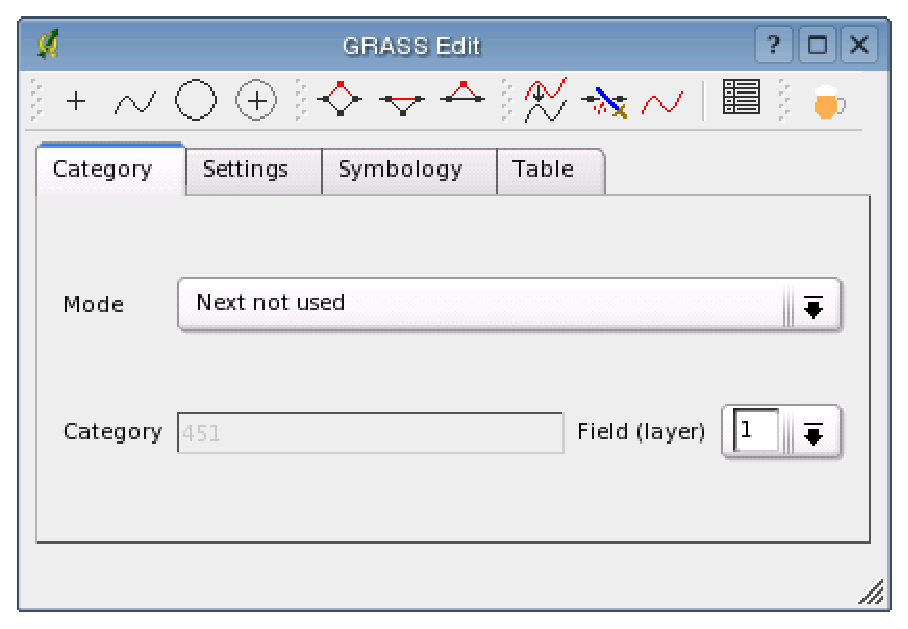
\includegraphics[scale=.7]{qgis_user_guide_images/grassedit}
\end{center}  
\end{figure}
The tools and settings are discussed in the following sections.\\
\subsubsection{Toolbar}
Table \ref{tab:grass_tools} lists the digitizing tools provided by the GRASS plugin. These correspond to the tool buttons in the toolbar(s) across the top of the dialog.
\begin{table}[h]
\centering
\caption{GRASS Digitizing Tools}\label{tab:grass_tools}\medskip
 \begin{tabular}{|l|p{5in}|}
 \hline \textbf{Tool} & \textbf{Purpose} \\
\hline New Point & digitize new point \\
\hline New Line &  digitize new line (finish by selecting new tool) \\
\hline New Boundary & digitize new boundary (finish by selecting new tool)\\
\hline New Centroid & digitize new centroid (label existing area)\\
\hline Move vertex & select one vertex of existing line or boundary and identify new position\\
\hline Add vertex & add a new vertex to existing line\\
\hline Delete vertex & delete one vertex from existing line (confirm selected vertex by another click)\\
\hline Move line & select existing line and click on new position\\
\hline Split line & split an existing line to 2 parts\\
\hline Delete line & delete existing line (confirm selected line by another click)\\
\hline Edit attributes & edit attributes of existing element (note that one element can represent more features, see above)\\
\hline Mug & close digitizing session\\
\hline
\end{tabular}
\end{table}
\subsubsection{Category Tab}
This tab allows you to set the way in which the category will be assigned to each new feature and/or assign a category to a feature.
\begin{compactitem}
\item Mode: what category should be attached to geometry
\begin{compactitem}
\item Next not used - next category not yet used in vector
\item Manual entry - define the category in 'Category entry'
\item No category - digitize geometry without category
\end{compactitem}
\item Category - a number (ID) attached to digitized feature
\item Field - feature (attribute table) identification
\end{compactitem}
\subsubsection{Settings Tab} 
This tab allow you to set the snapping in screen pixels. This is the threshold in pixels in which new points or line ends are snapped to existing nodes. This helps prevent gaps or dangles between boundaries

\subsubsection{Symbology Tab}
This tab allows you to view and set symbology for various geometry types and their topological status (e.g. closed / opened boundary).

\subsubsection{Table} 
This tab provides the means to view, create, or modify the database table for a given field.
\begin{Tip}\caption{\textsc{GRASS Edit Permissions}}
\qgistip{You must be the owner of the GRASS mapset you want to edit. It is impossible to edit vectors in mapsets which are not yours, even if you have write permissions.
}
\end{Tip} 

\subsubsection{Region Tool}

The current region (window) in GRASS is very important for all 
raster modules. All new created rasters have the extension and resolution
of the current region, regardless their original region. 
The region is stored in \$LOCATION/\$MAPSET/WIND file, and it defines
north, south, east, west, number of columns, number of rows, 
horizontal and vertical resolution.\\

It is possible to switch on/off the grass region in QGIS canvas
using the \textsl{Display Current GRASS Region} button.\\

With the \textsl{Edit Current GRASS Region} you can open a tool 
in which you can change the current region and symbology
of the rectangle on the QGIS Canvas. When the tool is running,
it is also possible to select a new region interactively
on the QGIS canvas.\\

Both tools are available only if QGIS was started from a GRASS 
shell or if the GISRC enviroment variable pointing to a
valid GISRC file was set (i.e. only if you are running 
GRASS within your mapset).

%\subsection{The GRASS Toolbar}
%The GRASS toolbar is displayed when the GRASS plugin is loaded using the Plugin Manager (see Section \ref{sec:managing_plugins}, \textsl{Managing Plugins}). Figure  shows the toolbar with each function annotated.

\section{Using Plugins}
QGIS has been designed with a plugin architecture. This allows new features/functions to be added to the application. Many of the features in QGIS are actually implemented as plugins.\\

There are two types of plugins in QGIS: core and user-contributed. A core plugin is maintained by the QGIS development team and is part of every QGIS distribtution. A user-contributed plugin is an external plugin that is maintained by the individual author. The QGIS Community site (\url{http://community.qgis.org}) serves as the repository for user contributed plugins.

\subsection{Finding and Installing a Plugin}
When you install QGIS, all of the core plugins are included (these are described below). Additional user-contributed plugins may be available on the QGIS Community site. To see what user-contributed plugins are available, see the plugins page on the Community site (\url{http://community.qgis.org/plugins}).\\

Typically user-contributed plugins are distributed in source form and require compiling. For instructions on building and installing a user-contributed plugin, see the documentation included with the plugin.
\subsection{Managing Plugins}\label{sec:managing_plugins}
Managing plugins consists of loading or unloading them from QGIS. Loaded plugins are "remembered" when you exit the application and restored the next time you run QGIS.\\

To manage plugins, open the \textsl{Plugin Manager} from the \textsl{Tools} menu. The Plugin Manager displays all the available plugins and their status (loaded or unloaded). Figure \ref{fig:pluginmanager} shows the Plugin Manager dialog.

\begin{figure}[h]
   \begin{center}
   \caption{Plugin Manager}\label{fig:pluginmanager}\smallskip
   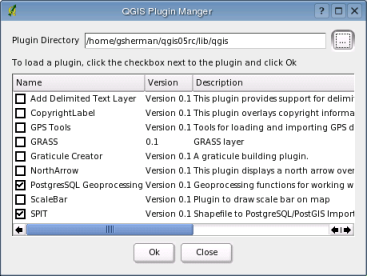
\includegraphics{qgis_user_guide_images/pluginmanager_80pct}
\end{center}  
\end{figure}
Typically all QGIS plugins are installed in the same location. This location is shown in the Plugin Directory text field. You can tell QGIS to load plugins from another location by specifying a different directory.
\begin{Tip}\caption{\textsc{Crashing Plugins}}
\qgistip{If you find that QGIS crashes on startup, a plugin may be at fault. You can stop all plugins from loading by editing your .qt/qgisrc file in your home directory on Linux/Unix (Windows users will have to edit the registry). On Linux/Unix, open the qgisrc file in a text editor and find the [Plugins] section. Set all the plugin values to false to prevent them from loading. For example, to prevent the Delimited text plugin from loading, the entry in qgisrc should look like this:\ttfamily{
 Add Delimited Text Layer=false}.\normalfont  Do this for each plugin in the [Plugins] section. You can then start QGIS and add the plugins one at a time from the Plugin Manger to determine which is causing the problem.

}
\end{Tip} 

\subsection{Data Providers}
Data Providers are "special" plugins that provides access to a data store. By default, QGIS supports PostGIS layers and disk-based data stores supported by the OGR library (Appendix \ref{appdx_ogr}). A Data Provider plugin extends the ability of QGIS to use other data sources.\\

Data Provider plugins are registered automatically by QGIS at startup. They are not managed by the Plugin Manager but are used behind the scenes when a corresponding data type is added as a layer in QGIS.
\subsection{Core Plugins}
QGIS currently contains 9 core plugins that can be loaded using the Plugin Manager. Table \ref{tab:core_plugins} lists each of the core plugins along with a description of their purpose. Figure \ref{fig:plugintoolbar} shows the icon for each plugin in the Plugin toolbar (the number corresponds to the Item in Table \ref{tab:core_plugins}. Note the GRASS plugin is not included below because it installs its own toolbar (see Section \ref{sec:grass} for a discussion of available features in GRASS plugin).
\begin{table}[h]
\centering
\caption{QGIS Core Plugins}\label{tab:core_plugins}\medskip
\small
 \begin{tabular}{|l|l|p{4in}|}
\hline \textbf{Item} & \textbf{Plugin} & \textbf{Description} \\
\hline 1 & Copyright Label & Display a copyright label on the map canvas\\
\hline 2 & Delimited Text & Load a delimited text file containing x,y coordinates as a point layer \\
\hline 3 & GPS Tools & Load and display GPS data \\
\hline 4 & Graticule Creator & Create a latitude/longitude grid and save as a shapefile\\
\hline 5 & Scalebar & Add a scalebar to the map canvas\\
\hline 6 & North Arrow & Add a north arrow to the map canvas\\
\hline 7 & PostgreSQL Geoprocessing & Buffer a PostGIS layer \\
\hline 8 & SPIT & Shapefile to PostGIS Import Tool - import shapefiles into PostgreSQL\\
\hline
\end{tabular}
\end{table}
\normalsize
\begin{figure}[h]
   \begin{center}
   \caption{Plugin Toolbar and Icons}\label{fig:plugintoolbar}\smallskip
   
\includegraphics[scale=1.0]{qgis_user_guide_images/plugintoolbar}
\end{center}  
\end{figure}
\clearpage
\appendix
\section{Supported OGR Formats}\label{appdx_ogr} 
At the data of this document, the following formats are supported by the OGR library.
\begin{compactitem}
\item Arc/Info Binary Coverage
\item Comma Separated Value (.csv) 
\item DODS/OPeNDAP
\item ESRI Shapefile
\item FMEObjects Gateway
\item GML
\item IHO S-57 (ENC)
\item Mapinfo File
\item Microstation DGN
\item OGDI Vectors
\item ODBC
\item Oracle Spatial
\item PostgreSQL\footnote{QGIS implements its own PostgreSQL functions. OGR should be built without PostgreSQL support}
\item SDTS
\item SQLite
\item UK .NTF
\item U.S. Census TIGER/Line
\item VRT - Virtual Datasource
\end{compactitem}
\section{GDAL Raster Formats}\label{appdx_gdal}
At the date of this document, the following formats are supported by the GDAL library. Note that not all of these format may work in QGIS for various reasons. For example, some require external commercial libraries. Only those formats that have been well tested will appear in the list of file types when loading a raster into QGIS. Other untested formats can be loaded by selecting the \textsl{All other files (*)} filter. Formats known to work in QGIS are indicated in \textbf{bold}.

\begin{compactitem}
\item \textbf{Arc/Info ASCII Grid}
\item \textbf{Arc/Info Binary Grid (.adf)}
\item Microsoft Windows Device Independent Bitmap (.bmp)
\item BSB Nautical Chart Format (.kap)
\item VTP Binary Terrain Format (.bt)
\item CEOS (Spot for instance)
\item First Generation USGS DOQ (.doq)
\item New Labelled USGS DOQ (.doq)
\item Military Elevation Data (.dt0, .dt1)
\item ERMapper Compressed Wavelets (.ecw)
\item ESRI .hdr Labelled
\item ENVI .hdr Labelled Raster
\item Envisat Image Product (.n1)
\item EOSAT FAST Format
\item FITS (.fits)
\item Graphics Interchange Format (.gif)
\item \textbf{GRASS Rasters}\footnote{GRASS raster support is supplied by the QGIS GRASS data provider plugin} 
\item \textbf{TIFF / GeoTIFF (.tif)}
\item Hierarchical Data Format Release 4 (HDF4)
\item \textbf{Erdas Imagine (.img)}
\item Atlantis MFF2e
\item Japanese DEM (.mem)
\item \textbf{JPEG JFIF (.jpg)}
\item JPEG2000 (.jp2, .j2k)
\item JPEG2000 (.jp2, .j2k)
\item NOAA Polar Orbiter Level 1b Data Set (AVHRR)
\item Erdas 7.x .LAN and .GIS
\item In Memory Raster
\item Atlantis MFF
\item Multi-resolution Seamless Image Database  MrSID
\item NITF
\item NetCDF
\item OGDI Bridge
\item PCI .aux Labelled
\item PCI Geomatics Database File
\item Portable Network Graphics (.png)
\item Netpbm (.ppm,.pgm)
\item \textbf{USGS SDTS DEM (*CATD.DDF)}
\item SAR CEOS
\item \textbf{USGS ASCII DEM (.dem)}
\item X11 Pixmap (.xpm)

\end{compactitem}

\end{onehalfspace}

\end{document}
